\section{Challenges}
% We had to resolve several challenges while trying to generate a satisfiable DOM tree.

\header{Single DOM Clues are Incomplete.}  
% why tracing, not greedy
Each DOM operation provides a clue to the overall DOM tree.  An intuitive approach would be to generate DOM elements "just in time".  
However, such naïve approach does not always work because each clue by itself is insufficient.  

Just in time generation is to greedily create whatever DOM elements necessary for satisfying the current single DOM clue.  
For example, in Sample Code \ref{dom0}, whenever {\tt getElementById()} is called, we could just create and return an ad-hoc DOM element having the corresponding id.  
When we see {\tt (row.children.length === 10)}, we could additionally create 10 ad-hoc children for the {\tt row}.  

The problem is that other DOM operations may contradict the ad-hoc DOM tree.  
A counter example we discovered very early is by just loading Wikipedia~\cite{wikipedia}.  
While loading the webpage, it executes the jQuery {\tt \$("\#B13\_120517\_dwrNode\_enYY")}, which is to get an element by a specific id.  
Then, some time later, the webpage calls {\tt \$("div\#B13\_120517\_dwrNode\_enYY")}, which is to get a <div> element by the exact same id.  
While the two jQueries may be written by different developers, we can easily see that the greedy approach does not work because it does not consider DOM operations in other parts of the code.  

While each DOM clue is incomplete, there can also be many different possibilities for satisfying a single DOM clue.  
When trying to satisfy {\tt \$("\#B13\_120517\_dwrNode\_enYY")}, the DOM has so many tag types, how do we know <div> is the correct tag in the first place?  
The consequence for an incorrect tag type is that the 2nd jQuery would not return any DOM element, leading to an error.  
Thus DOM operations have to be collectively traced for complete analysis and for generating a correct answer.  


\header{Intermediate Variables.}  
% why backward slicing
While executing JavaScript code would subtly or passively imply the DOM having a particular tree structure (as in the jQuery example), sometimes the structure of the DOM tree would actively determine which branch a condition would go into.  
For example, in Sample Code~\ref{dom0}, we see that whether a {\tt row} has 10 children would actively determine whether the {\tt if} condition would go into the {\tt true} or {\tt false} branch.
While the DOM dependence is obvious in Sample Code~\ref{dom0}, very often DOM operations may not directly appear inside a condition: the result of different DOM operations may get assigned to multiple variables at various execution stages prior to the condition, either within the same function or up in the runtime stack.  
For example, a condition may appear as a simple {\tt if(a)} in the code; yet the variable {\tt a} can be {\tt (row.children.length === 10)} or something more complex, such as the result of multiple statements executed throughout the code.  
We have to backward slice variables so that we can accurately determine what DOM operations a condition may depend upon.  


\header{Dynamic Typing.}  
% why dynamic analysis, not static analysis; why tracing and backward slicing both have to be dynamic.
JavaScript variables are dynamically typed.  Thus given a variable, we won't know exactly what type its value represents until we actually run the code.  
In our previous example, {\tt a} can be anything: an integer, a string, a boolean, or an object.  
Static analysis by itself is insufficient to detect which lines of code are DOM related.
Indeed, authors of existing JavaScript static techniques~\cite{staticJsWWW09, staticJsWWW11} reveal substantial gaps and false positives in their own work.  
Thus the only way to discover whether a condition contains DOM operations is to run the code.  Both tracing and backward slicing have to be dynamic to accurately determine which conditions depend on the DOM, and which don't.  

%What is the best and simplest way to incorporate dynamic tracing and dynamic backward slicing into the execution of JavaScript source code?  
%After all, if we were to support concolic testing, we must be able to accurately guide execution towards an intended path and thus we must properly understand how a condition would result in the {\tt True} and {\tt False} branches.    
%As stated in our contributions, our approach is generic, transparent, and browser independent; thus we cannot modify the source code of Web browsers and natively support slicing and tracing.  
%This is why we instrument JavaScript as it gets downloaded to the browser.  
% why decorated execution, not offline analysis 
%Adding to the overall complexity, conditions are usually composed of sub-conditions linked by logical operators (e.g. {\tt or}'s, {\tt and}'s, {\tt not}'s) nested inside one another.
%Executions of conditions can also have precedence.  For example, in an {\tt and}, when the first sub-condition is {\tt false}, the second sub-condition is never executed.  Similarly, an {\tt or} never executes the second sub-condition when the first returns {\tt true}.
% how is this a challenge
% drives the need for decorated execution, different from Jalangi

\begin{figure}
\begin{lstlisting}[caption=Example code showing DOM operations can have logical constraints that are interdependent with each other.  To make both of these {\tt if} statements true sub conditions i) and ii) become mutually exclusive: they cannot be true at the same time.  Thus a logic solver is required to generate a satisfiable DOM structure and HTML.,label=domOr]  
// Interdependent Logic
// ...
if (d === elem.firstElementChild // i)
 || d === b.lastElementChild) {}
// ... 
if (d === elem.parentElement // ii)
 || d === b.parentElement) {}
// ...
if (b.previousElementSibling === 
    c.firstElementChild) {}
// ... 
if (elem.parentElement.parentElement 
    === c.lastElementChild.previousElementSibling) {}  
// ... 
\end{lstlisting}
\end{figure}


\header{Interdependent Logic}  
% why solver, not heuristics 
Given a dynamic trace and a dynamic backward slice deduced from the logs of decorated execution, we would have a clear mapping between DOM operations and conditions; thus a logical approach would be to generate a DOM tree directly from the trace and backward slice.  
However, an heuristic approach may not always work because a condition may have logical constraints that are interdependent on logical constraints in other conditions.  
In an obvious example, 2 of the conditions in Sample Code~\ref{domOr}, the 2 {\tt if} statements, inter-depend on each other because of the DOM policy that a DOM element cannot be both a child and a parent of another DOM element.  
Specifically, sub-conditions {\tt i} and {\tt ii} must be mutually exclusive because {\tt d} cannot be both a child and parent of {\tt a}.
Therefore, when we want both of these {\tt if} conditions to be {\tt true}, a DOM specific solver is required to understand the unique policies of the DOM and make decisions accordingly for generating a proper satisfying HTML.


\begin{figure*}[ht]
\centerline{\scalebox{1.0}{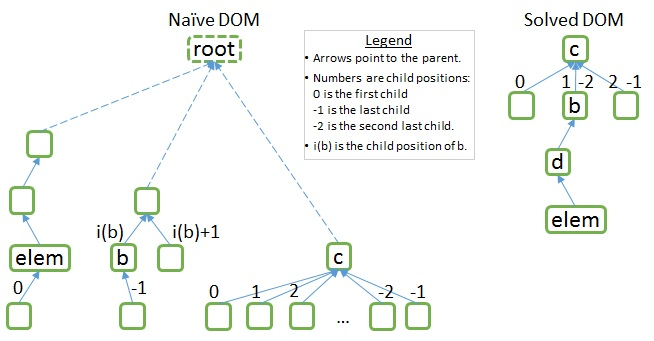
\includegraphics[natwidth=654,natheight=341]{trees.jpg}}}
\caption[Naive vs. Solved DOM trees]{An na\"{i}ve and the solver approach to generating a satisfiable DOM.  The naive DOM attempts and fails to the DOM operations by simply sorting individual DOM clues by element and connecting them with a single root (dashed lines).  In the Solved DOM {\tt b} is both child 1 (seocnd child) and child -2 (last child's previous sibling).  {\tt elem} does not have any child because {\tt elem.firstElementChild} is actually in an {\tt or} clause (Sample Code ~\ref{domOr}), in which the solver has decided to make the other sub clause {\tt true}.}
\label{trees}
\end{figure*}


\header{2D Tree Structure \& Implicit Clues.}  
% why quantifiers and not meshing tree pieces together
The DOM solver must also be able to infer indirect clues based on the 2D tree structure of the DOM.  For example, when {\tt b.previousElementSibling === c.firstElementChild}, the solver has to understand the implication that {\tt c} is the parent of {\tt b}.  

The DOM solver also has to consider the fact that the DOM clues can subtly overlap with each other.  DOM clues can overlap because DOM operations can be chained.  In JavaScript, a DOM operation of a DOM element (e.g. {\tt elem.parentElement}) returns another DOM element.  Thus DOM operations can be chained: {\tt elem.parentElement.parentElement}.  
In Figure~\ref{trees}, when {\tt elem.parentElement.parentElement === c.lastElementChild.previousElementSibling}, the subtle implication is that {\tt b.nextElementSibling} is {\tt c.lastElementChild}, because {\tt d === b.parentElement} and {\tt d === b.lastElementChild}.  

Overlapping can become complex after the intermediate variables are resolved into a long dynamic backward slice.  The reason is that, there can be multiple long chains in both parental and sibling dimensions: e.g. {\tt elem.parentElement.parentElement.nextElementSibling.children[2]}.  
The multiple long chains can overlap and weave with each other on multiple spots.
Thus the 2D structure and indirect clues are another reason for requiring a DOM specific solver.  A non-solver approach would simply not work when it tries to generate a naïve tree (Naïve DOM in Figure \ref{trees}) by grouping the DOM operations and then connecting the individual tree pieces to a master root (the dashed lines in Figure \ref{trees}).  


% \header{DOM Mutations}  
% give update score as example
% why conditional slicing
% why 2D is more challenging than 1D
%Expressing the DOM for a solver is not as easy as expressing single dimensional numerical or string operations (e.g. additions and subtractions), because no solver supports 2D tree structures natively and DOM operations are more diverse.  
%Mutations to the DOM tree structure must also be accounted for in both the backward slicing and the solver because changes to the HTML can happen any time during execution.  
%Example mutations include adding or deleting a DOM element (e.g. in the use case of refreshing an email Inbox or deleting a message), or modifying the content or attributes within a DOM element.  
